\documentclass[11pt]{article}

\usepackage[margin=1in]{geometry}

\usepackage{amsmath,amssymb,amsthm,mathtools}
\usepackage{graphicx}
\usepackage{booktabs}
\usepackage{adjustbox}
\usepackage[section]{placeins}
\usepackage{xcolor}
\usepackage[expansion=false]{microtype}
\usepackage{enumitem}
\usepackage[font=small,labelfont=bf]{caption}
\usepackage[ruled,vlined,linesnumbered]{algorithm2e}
\usepackage{tikz}
\usetikzlibrary{positioning,arrows.meta,calc}
\usepackage[most]{tcolorbox}
\usepackage[numbers,sort&compress]{natbib}
\usepackage[colorlinks=true,linkcolor=blue!50!black,citecolor=blue!50!black,urlcolor=blue!50!black]{hyperref}
\usepackage[capitalise,noabbrev]{cleveref}

\input{tables/dates.tex}
\input{tables/numbers.tex}

\newtheorem{theorem}{Theorem}
\newtheorem{proposition}[theorem]{Proposition}
\newtheorem{corollary}[theorem]{Corollary}
\newtheorem{lemma}[theorem]{Lemma}
\theoremstyle{definition}
\newtheorem{definition}{Definition}
\newtheorem{example}{Example}
\theoremstyle{remark}
\newtheorem{remark}{Remark}

\newtcolorbox{plainwords}[1][]{colback=blue!3!white,colframe=blue!40!black,boxrule=0.5pt,
  arc=2pt,left=6pt,right=6pt,top=4pt,bottom=4pt,fonttitle=\bfseries\small,title={In plain words#1}}

\newcommand{\R}{\mathbb{R}}
\newcommand{\C}{\mathbb{C}}
\newcommand{\ip}[2]{\langle #1, #2 \rangle}
\newcommand{\tr}{\operatorname{tr}}
\newcommand{\diag}{\operatorname{diag}}
\newcommand{\one}{\mathbf{1}}
\newcommand{\pnl}{\bar{\pi}}
\newcommand{\Proj}{\mathcal{P}}
\DeclareMathOperator{\Real}{Re}
\DeclareMathOperator{\Imag}{Im}

\title{Rank-Preserving Synthetic Returns for Linear Signal Strategies:\\
A Ladder of Invariances for Robustness Testing}
\author{Nicholas Sambelashvili\\
\small Head of Quant Research, Limex FinTech}
\date{\small Draft --- \today}

\begin{document}
\maketitle

\begin{abstract}
Synthetic return paths are widely used to stress-test trading strategies, but the usual generators
(bootstrap, GARCH-type models, generative networks) are judged by how realistic the paths look, not
by which conclusions about strategies they leave intact. We propose to specify that invariance first.
A \emph{rung} is a class of strategies together with the set of data transformations that leave the
performance ranking of every strategy in the class unchanged; everything else about the data is free to vary.
For linear signal strategies $w_t=\sum_k A_k r_{t-k}$ with $\|A\|=1$, ranked by mean P\&L, we show that a subclass
preserves its rankings if and only if the projection of the lagged cross-moment matrices onto the subclass is
preserved up to scale, and that useful intermediate rungs must therefore be linear subspaces. In the frequency domain
each rung corresponds to a group of per-frequency unitary transformations, which yields a lattice of five
cross-sectional rungs (full, symmetric, factor, diagonal, pooled) that can be combined with frequency bands.
We give a generator that samples from each rung exactly, while also pinning the mean and covariance matrix and
restoring fat tails and volatility clustering. On twenty years of daily returns for 97 US instruments and for the
nine sector ETFs, every rung reproduces the rankings of its own strategy class exactly, whereas block bootstrap and
VAR surrogates reach a Kendall $\tau$ of only 0.5--0.7, GARCH surrogates about zero, and classical Fourier surrogates lose tails or volatility clustering.
Used as a ladder of null hypotheses, the rungs give an \emph{edge profile} that locates the structure a strategy
exploits. Applied to standard momentum and reversal strategies, it shows that momentum P\&L is fully explained by
own-asset autocovariance, while the profit of one-week reversal is concentrated in high-volatility episodes, a
nonlinear feature that a volatility-normalized implementation largely fails to capture.
\end{abstract}

% =====================================================================
\section{Introduction}
\label{sec:intro}

A backtest is a single draw. Every trading strategy is evaluated on the one historical path the market happened to
produce, and it is well understood that this invites overfitting and false discoveries
\citep{bailey2014,harvey2016,lopezdeprado2018}. A natural response is to generate many synthetic paths and ask
whether a strategy's performance survives on them. The difficulty is that ``survives'' depends entirely on what the
synthetic paths keep from the original. A stationary bootstrap keeps fat tails and short-range dependence; a GARCH
simulation keeps volatility clustering; a generative network keeps whatever its loss function rewards. None of them
comes with a statement of the form \emph{``for these strategies, the synthetic data will give exactly the same answer
as the real data''}. Without such a statement, a change in a strategy's performance on synthetic data cannot be
attributed to anything specific.

This paper turns the question around. Instead of building a realistic generator and then checking what it preserves,
we first state which strategy comparisons must be preserved, and then let the generator vary everything else.
We call such a specification a \emph{rung}, as in the rung of a ladder:
\begin{itemize}[leftmargin=*,itemsep=2pt]
  \item a low rung protects few comparisons and leaves the synthetic data much freedom;
  \item a high rung protects many comparisons and leaves little freedom;
  \item at the top of the ladder only the original data protects every comparison.
\end{itemize}
Climbing the ladder with a strategy tells us at which point its performance becomes stable, and therefore which
features of the data it actually relies on.

\begin{plainwords}
Think of a rung as a contract between the synthetic data and the analyst: \emph{``ask me any question from this list
and I will give exactly the same answer as history; ask anything else and my answer may differ.''} The list of questions
is a family of strategies, and ``the answer'' is how those strategies rank against each other.
\end{plainwords}

We work out this idea for the class of \emph{linear signal strategies}, in which today's position in each asset is a
linear combination of past returns of all assets. This class contains time-series and cross-sectional momentum,
short-term reversal, lead--lag trades and factor momentum \citep{jegadeesh1993,lo1990,moskowitz1999,moskowitz2012}. Our contributions are:
\begin{enumerate}[leftmargin=*,itemsep=2pt]
  \item \textbf{A precise notion of rung} (\cref{sec:rungs}) and a characterization theorem: a subclass of linear signal
  strategies keeps its rankings if and only if a specific projection of the lagged cross-moment matrices is kept
  (\cref{thm:main}). A corollary shows that natural-looking shape restrictions such as rank-one strategies are as
  demanding as the full class (\cref{prop:rankone}), so useful intermediate rungs must be subspaces.
  \item \textbf{A frequency-domain construction} (\cref{sec:freq}) in which each rung corresponds to a group of
  per-frequency unitary transformations. This gives a lattice of five cross-sectional rungs that can be mixed across
  frequency bands.
  \item \textbf{A generator} (\cref{sec:generator}) that samples paths on any rung exactly, while also pinning the mean and
  covariance matrix and restoring fat tails and volatility clustering.
  \item \textbf{An empirical study} (\cref{sec:empirical}) on twenty years of daily data, with five baseline generators, and an
  \textbf{edge profile} application (\cref{sec:edge}) that locates the structure behind momentum and reversal profits.
\end{enumerate}
Code to reproduce every table and figure is released with the paper (see the code availability statement at the end).

% =====================================================================
\section{Related work}
\label{sec:related}

\paragraph{Surrogate data.} The idea of generating data that share chosen statistics with an observed series, and
using them as a null hypothesis, comes from nonlinear time-series analysis. \citet{theiler1992} introduced Fourier
phase randomization to test for nonlinearity; \citet{prichard1994} extended it to several simultaneously measured
series by applying a common random phase, which preserves all auto- and cross-spectra.
\citet{schreiber1996} proposed the iterative amplitude-adjusted Fourier transform (IAAFT), which also preserves each
series' marginal distribution, and \citet{schreiber1998} formulated surrogate generation as constrained randomization:
any set of statistics can be imposed by minimizing a cost function over permutations. A survey is \citet{schreiber2000}.
Our full rung is, at its core, the multivariate phase randomization of \citet{prichard1994}; the contribution here is the
lattice of weaker rungs, the link between each rung and a strategy class, and the additional covariance, tail and
volatility steps.

\paragraph{Resampling and parametric simulation.} Block and stationary bootstraps \citep{kunsch1989,politis1994}
resample stretches of history and keep local dependence. GARCH models \citep{bollerslev1986}, with constant conditional
correlation \citep{bollerslev1990} and filtered historical simulation \citep{baroneadesi1999}, are standard in risk
management. Generative networks such as Quant GANs \citep{wiese2020} learn the path distribution directly.
\citet{lopezdeprado2018} discusses synthetic data for backtesting. These methods aim at realism; we use several of them as
baselines and show that they do not preserve strategy rankings.

\paragraph{Return predictability.} \citet{lo1990} decomposed contrarian profits into three terms: own autocovariance,
cross autocovariance and the dispersion of mean returns; their decomposition is a special case of the inner product
$\ip{A}{M}$ that underlies our analysis, and our diagonal rung generalizes it (\cref{sec:edge}). The multivariate
portmanteau statistic \citep{hosking1980} measures the total size of the lagged correlation matrices that linear
strategies trade on. The dependence of short-term reversal profits on market volatility is documented by
\citet{nagel2012}; volatility-managed portfolios are studied by \citet{moreira2017}.

% =====================================================================
\section{Rungs: which comparisons does synthetic data keep?}
\label{sec:rungs}

\subsection{Setting and definition}

Let $r_t\in\R^N$, $t=0,\dots,T-1$, be daily returns of $N$ instruments, collected in the $T\times N$ matrix $R$.
A \emph{strategy} maps the history to positions $w_t\in\R^N$ and earns $\pi_t=w_t^\top r_t$. A \emph{performance
metric} $\phi$ turns the P\&L series into a number, for example the mean or the Sharpe ratio.

\begin{definition}[Rung]\label{def:rung}
Let $\mathcal{S}$ be a set of strategies and $\phi$ a metric. A data set $R'$ is \emph{$(\mathcal{S},\phi)$-equivalent}
to $R$ if, for all $a,b\in\mathcal{S}$,
\[
  \phi_R(a) > \phi_R(b) \iff \phi_{R'}(a) > \phi_{R'}(b).
\]
The \emph{rung} of $(\mathcal{S},\phi)$ is the set of all data sets equivalent to $R$. A \emph{rung generator} draws random elements of a rung.
\end{definition}

Two consequences are immediate. First, enlarging $\mathcal{S}$ shrinks the rung: more comparisons must be kept, so fewer
data sets qualify. Nested strategy classes therefore give nested rungs, a ladder. Second, a rung says nothing about
strategies outside $\mathcal{S}$. Their rankings may change, and that freedom is precisely what makes the synthetic data
informative.

\subsection{A warm-up: the static ladder}
\label{sec:static}

Before turning to signals, consider \emph{static} portfolios: fixed weights $w$, rebalanced daily.
\begin{itemize}[leftmargin=*,itemsep=2pt]
  \item \textbf{Ranked by mean return}, $\phi(w)=w^\top\mu$. The ranking of all $w$ is kept if and only if the mean vector
  is kept up to a positive scale. Covariances, tails and dynamics are all free.
  \item \textbf{Ranked by Sharpe ratio}, $\phi(w)=w^\top\mu/\sqrt{w^\top\Sigma w}$. One needs, essentially, $\mu$ and
  $\Sigma$ up to scale. Everything beyond the first two moments is free.
  \item \textbf{Ranked by any metric that ignores time order} (compounded return, volatility, CVaR, skewness, \dots). One needs
  the empirical distribution of the daily return vectors. Only the order of the days is free, so the rung consists of the
  date permutations.
  \item \textbf{Weights allowed to change at the boundaries of calendar blocks of length $B$.} Only permutations of days within each
  block survive. As $B\to 1$, the strategy ``hold asset $i$ only on day $t$'' isolates every single return, and only the
  original data remains.
\end{itemize}

\begin{example}[Three assets, Sharpe ranking]
Take stock, bond and gold with annual means $\mu=(8\%,3\%,5\%)$ and some covariance matrix $\Sigma$. A synthetic data set in
the Sharpe rung must reproduce $\mu$ and $\Sigma$ (up to a common scale), so every portfolio, for instance 60/40 stock/bond or
1/3 each, has the same Sharpe ratio as in history and keeps its place in the league table. The synthetic data may, however, put
the 2008 crash in 2015, make gold's tails fatter, or remove volatility clustering. A strategy that needs any of these
features to look good is therefore not a static mean--variance strategy, and the Sharpe rung will reveal this.
\end{example}

The rest of the paper does the same for strategies whose weights respond to past returns. Every generator we build
also keeps $\mu$ and $\Sigma$ exactly, so each signal rung sits on top of the static Sharpe rung.

\subsection{Linear signal strategies}

A \emph{linear signal strategy} with lookback $L$ is a stack $A=(A_1,\dots,A_L)$ of $N\times N$ matrices and positions
\begin{equation}\label{eq:strategy}
  w_t=\sum_{k=1}^{L} A_k\,r_{t-k}.
\end{equation}
Row $i$ of $A_k$ says how the position in asset $i$ responds to the returns of all assets $k$ days ago. The P\&L is
$\pi_t=\sum_k r_t^\top A_k r_{t-k}=\sum_k \tr\!\big(A_k^\top r_t r_{t-k}^\top\big)$, so the mean P\&L is
\begin{equation}\label{eq:pnl}
  \pnl(A)=\frac1T\sum_t \pi_t=\sum_{k=1}^{L}\ip{A_k}{M_k},\qquad
  M_k=\frac1T\sum_{t} r_t\,r_{t-k}^\top,
\end{equation}
where $\ip{P}{Q}=\tr(P^\top Q)$ is the Frobenius inner product. The matrix $M_k$ collects all lag-$k$ cross-moments:
its entry $(i,j)$ is the average of ``today's return of $i$ times the return of $j$ $k$ days ago''.
Throughout, time indices are taken modulo $T$ (a \emph{circular} sample); \cref{sec:limits} discusses the difference from an
ordinary backtest. Because doubling $A$ doubles the P\&L, we compare strategies at a fixed size, $\|A\|_F=1$.

Familiar strategies are particular choices of $A$ (with $I$ the identity and $J=\one\one^\top/N$ the averaging matrix):
\begin{center}
\small
\begin{tabular}{ll}
\toprule
Strategy & $A_k$ \\
\midrule
Time-series momentum (each asset follows its own past) & $I$ \\
Cross-sectional momentum (long past winners, short past losers) & $I-J$ \\
Cross-sectional reversal \citep{lo1990} & $-(I-J)$ \\
Market timing / trend (all assets follow the market's past) & $J$ \\
Factor momentum (follow the past of $K$ factors $F$) & $FF^\top$ \\
Follow the leader (asset $i$ follows asset $j$) & $e_i e_j^\top$ \\
\bottomrule
\end{tabular}
\end{center}

\subsection{The main result}

\Cref{eq:pnl} says that all linear signal strategies are scored by a single object, the stack $M=(M_1,\dots,M_L)$, and that the score
is linear in $A$. This makes rungs easy to characterize.

\begin{theorem}[Rungs of linear signal strategies]\label{thm:main}
Let $V$ be a linear subspace of strategy stacks, $\mathcal{S}_V=\{A\in V:\|A\|_F=1\}$, and let $\Proj_V$ denote orthogonal projection
onto $V$. A data set $R'$ with lagged cross-moments $M'$ ranks $\mathcal{S}_V$ by mean P\&L exactly as $R$ does if and only if
\[
  \Proj_V M' = c\,\Proj_V M \quad\text{for some } c>0,
\]
or $\Proj_V M'=\Proj_V M=0$.
\end{theorem}

The proof is in \cref{app:proofs}. The intuition: on the unit sphere of $V$, the P\&L $\ip{A}{\Proj_V M}$ is a linear function, and a
linear function on a sphere is completely ranked by its direction. A rung for $V$ therefore pins $\dim V-1$ numbers (a direction)
and leaves all components of $M$ orthogonal to $V$ free, together with everything that is not a lagged second moment at all:
tails, volatility clustering, the timing of crashes.

One might hope to obtain intermediate rungs from shape restrictions, for example strategies that trade a single portfolio on a single
signal, $A_1=uv^\top$. This does not work:

\begin{proposition}[Shape classes pin their span]\label{prop:rankone}
Let $L=1$ and let $\mathcal{S}_1=\{uv^\top:\|u\|=\|v\|=1\}$ be the rank-one strategies. A data set ranks $\mathcal{S}_1$ exactly as $R$ does if
and only if $M_1'=cM_1$ for some $c>0$.
\end{proposition}

Rank-one strategies form a set of dimension $2N-1$, far smaller than the $N^2$ dimensions of all strategies, yet they pin all of $M_1$.
The reason is that their rankings already determine the sign of $u^\top M_1 v$ for every pair $(u,v)$, and these signs determine $M_1$ up to scale.
The same argument applies to separable strategies $A_k=h_kB$. The lesson is that \emph{useful rungs are subspaces}, and we build them that way.

\subsection{The five cross-sectional rungs, explained}
\label{sec:five}

We restrict each $A_k$ to lie in a subspace $W$ of $N\times N$ matrices, the same for every lag. By \cref{thm:main} the rung then pins the
projection of every $M_k$ onto $W$. We use five choices of $W$; \cref{fig:lattice} shows how they nest.

To make them concrete we use a toy market with two assets throughout. Asset X has mild momentum of its own; asset Y has
slight reversal of its own and, more importantly, \emph{follows} X with a one-day delay:
\[
  x_t = 0.10\,x_{t-1}+\varepsilon_t,\qquad y_t = 0.30\,x_{t-1}-0.05\,y_{t-1}+\eta_t .
\]
Its lag-one cross-moment matrix, with rows for today's return and columns for yesterday's, is
\[
  M_1=\begin{pmatrix} a & b\\ c & d\end{pmatrix}
  =\begin{pmatrix} \text{X after X} & \text{X after Y}\\ \text{Y after X} & \text{Y after Y}\end{pmatrix}.
\]
Here $a>0$ (X's own momentum), $d<0$ (Y's own reversal), $c>0$ large (X leads Y) and $b\approx 0$ (Y does not lead X).
\Cref{tab:toy} shows $M_1$ for a simulated sample of 4{,}000 days and for one synthetic path from each rung. We now go through the rungs from the
least to the most demanding.

\begin{table}[htbp]
\centering\small
\begin{adjustbox}{max width=\textwidth}\input{tables/tab_toy.tex}\end{adjustbox}
\caption{Toy two-asset market in which X leads Y. Rows: the original sample and one synthetic path from each rung (\cref{alg:generator}).
The market column is $f^\top M_1 f$ with $f=(1,1)/\sqrt2$, the lag-one autocovariance of an equal-weight portfolio. Each rung keeps exactly the
combinations it promises (pooled: $a+d$; diagonal: $a$ and $d$; symmetric: $a$, $d$ and $(b+c)/2$; factor: the market column; full: everything)
and lets the other entries move.}
\label{tab:toy}
\end{table}

\paragraph{Pooled rung: $W=\{\lambda I\}$.} Strategies: every asset is traded on its own past with \emph{the same} rule, for example
``buy whatever went up last month'' applied identically to all assets. Pinned: the average own-autocovariance $\tr M_k$, one number per lag.
Free: how that autocovariance is shared between assets, and all cross-asset effects.
\begin{plainwords}[: pooled]
In the toy market only $a+d$ is kept. A synthetic path may move all the momentum into Y and all the reversal into X, or weaken the
``X leads Y'' effect, as long as the average own-autocorrelation stays the same (\cref{tab:toy}: $c$ falls from 0.30 to 0.21).
A strategy that still looks good here only needs ``assets, on average, trend''.
\end{plainwords}

\paragraph{Diagonal rung: $W=\{\text{diagonal matrices}\}$.} Strategies: each asset is traded on its own past with its \emph{own} rule,
for example time-series momentum with asset-specific weights. Pinned: every asset's own autocovariance at every lag, $\diag M_k$.
Free: all lead--lag relations between different assets.
\begin{plainwords}[: diagonal]
Now $a$ and $d$ are both kept, but $b$ and $c$ are free. The synthetic path keeps X's momentum and Y's reversal and is free to destroy the
fact that X leads Y (in \cref{tab:toy}, $c$ drops from 0.30 to 0.19). If a cross-sectional strategy loses its edge on this rung, the edge came from
how assets predict \emph{each other}, not from how each asset predicts itself. This is the decomposition of \citet{lo1990}, made into a test.
\end{plainwords}

\paragraph{Symmetric rung: $W=\{A=A^\top\}$.} Strategies whose response is reciprocal: the position in $i$ reacts to $j$'s past exactly as
the position in $j$ reacts to $i$'s past. Cross-sectional momentum and reversal ($I-J$), market trend ($J$) and factor momentum ($FF^\top$) are all
symmetric. Pinned: the symmetric part $(M_k+M_k^\top)/2$. Free: the antisymmetric part $(M_k-M_k^\top)/2$, which is \emph{directional}
lead--lag (``$i$ predicts $j$ more than $j$ predicts $i$'').
\begin{plainwords}[: symmetric]
The total amount of cross-asset co-movement across days, $b+c$, is kept, but not its direction. A synthetic path may say ``Y leads X'' instead of ``X leads Y''.
The follow-the-leader strategy (buy Y after X rises, $A_1=e_Ye_X^\top$) is not symmetric, so its P\&L may change here, while every symmetric
strategy, such as ``long the pair after it rose'', keeps its P\&L.
\end{plainwords}

\paragraph{Factor rung: $W=\{FCF^\top\}$ for a fixed $N\times K$ factor matrix $F$ with orthonormal columns.} Strategies that both read signals
from, and take positions in, the $K$ factor portfolios, for example factor momentum on the leading principal components. Pinned: the lagged cross-moments
of the factors, $F^\top M_kF$ ($K^2$ numbers per lag). Free: everything idiosyncratic, i.e.\ orthogonal to the factors.
\begin{plainwords}[: factor]
With one factor, the equal-weight ``market'' $f=(1,1)/\sqrt2$, only $f^\top M_1 f=(a+b+c+d)/2$ is kept: how much the market as a whole trends.
Each individual entry may move (\cref{tab:toy}). A strategy that keeps its edge here only needs factor-level predictability; one that loses it
was trading the idiosyncratic part.
\end{plainwords}

\paragraph{Full rung: $W=\R^{N\times N}$.} All linear signal strategies. Pinned: every $M_k$. Free: everything that is not a lagged second
moment (tails, volatility clustering, nonlinear dependence, the dates of crashes).
\begin{plainwords}[: full]
Every number in $M_1$ is kept. The synthetic paths still look nothing like the original day by day (their correlation with the original path is about
zero), but no linear signal strategy can tell them apart from history. A strategy whose performance changes on this rung must be using something
beyond linear predictability, for example the interplay between volatility and predictability (\cref{sec:reversal}).
\end{plainwords}

\begin{figure}[htbp]
\centering
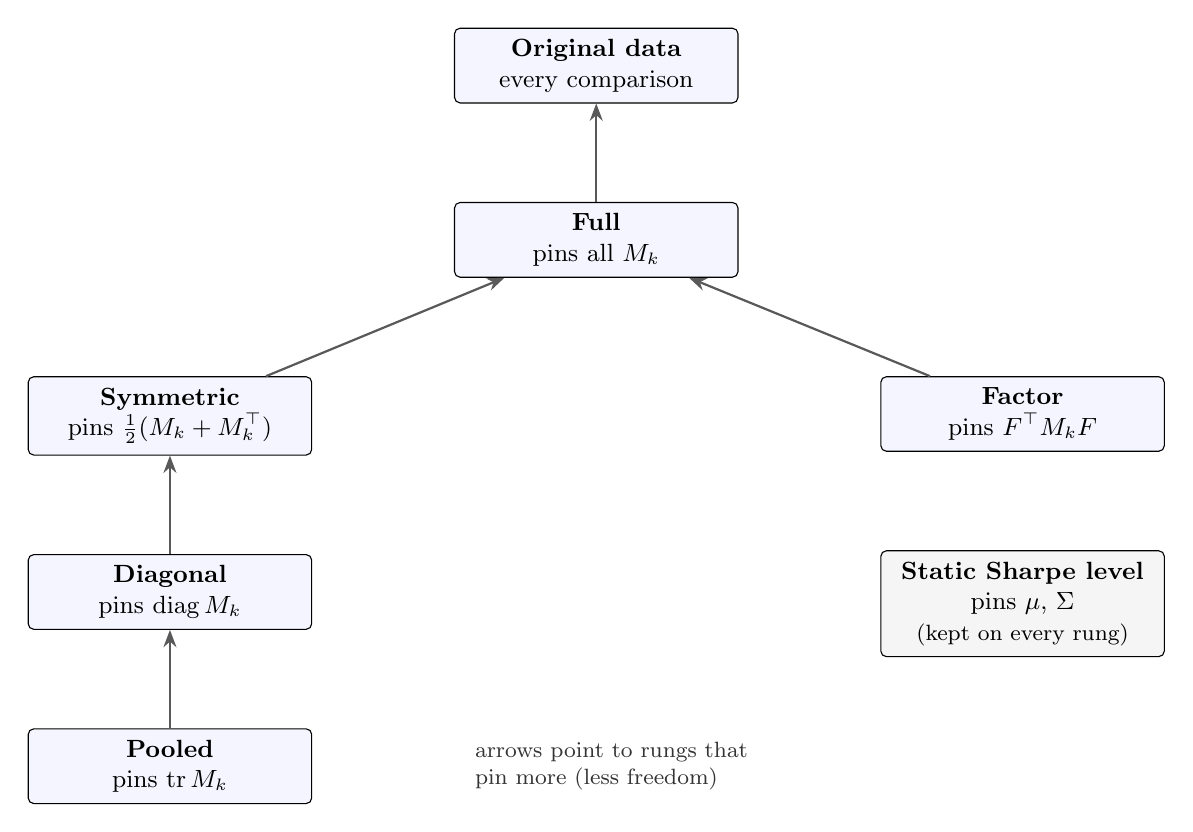
\begin{tikzpicture}[
  node distance=1.25cm and 1.8cm,
  box/.style={draw, rounded corners=2pt, align=center, font=\small, minimum width=3.6cm, inner sep=4pt, fill=blue!4},
  arr/.style={-{Stealth[length=2.2mm]}, thick, gray!70!black}]
  \node[box] (orig) {\textbf{Original data}\\ every comparison};
  \node[box, below=of orig] (full) {\textbf{Full}\\ pins all $M_k$};
  \node[box, below left=of full] (sym) {\textbf{Symmetric}\\ pins $\tfrac12(M_k+M_k^\top)$};
  \node[box, below right=of full] (fac) {\textbf{Factor}\\ pins $F^\top M_k F$};
  \node[box, below=of sym] (dia) {\textbf{Diagonal}\\ pins $\diag M_k$};
  \node[box, below=of dia] (poo) {\textbf{Pooled}\\ pins $\tr M_k$};
  \node[box, below=of fac, fill=gray!8] (stat) {\textbf{Static Sharpe level}\\ pins $\mu$, $\Sigma$ \\ \footnotesize(kept on every rung)};
  \draw[arr] (full) -- (orig);
  \draw[arr] (sym) -- (full);
  \draw[arr] (fac) -- (full);
  \draw[arr] (dia) -- (sym);
  \draw[arr] (poo) -- (dia);
  \node[font=\footnotesize, gray!40!black, align=left] at ($(poo.east)+(3.8,0)$) {arrows point to rungs that\\ pin more (less freedom)};
\end{tikzpicture}
\caption{The lattice of cross-sectional rungs. An arrow from rung $a$ to rung $b$ means that every data set on rung $b$ is also on rung $a$: the strategy
class of $b$ contains that of $a$. The factor rung is not comparable with the symmetric, diagonal or pooled rungs, because factor strategies $FCF^\top$
need not be symmetric, and $I$ is not of the form $FCF^\top$.}
\label{fig:lattice}
\end{figure}

\subsection{The second dial: which horizons}

The rungs above restrict how assets interact. Independently, one can restrict which \emph{horizons} are protected. A strategy with a 12-month
lookback reads slow movements of prices; a one-week reversal strategy reads fast ones. In the frequency domain (\cref{sec:freq}) this becomes a choice of
frequency band: a rung may pin the full cross-spectrum at low frequencies and only the pooled spectrum at high frequencies, for example.
Combining the cross-sectional choice $W$ with a band $\Phi$ gives a rung $W\otimes\Phi$, and the rungs form a lattice rather than a single chain.
Our experiments use the full band; \cref{sec:bands} explains the construction and its caveat for causal strategies.

% =====================================================================
\section{The frequency-domain construction}
\label{sec:freq}

\subsection{Strategies as filters}

Let $X_j=\sum_{t=0}^{T-1} r_t\,e^{-2\pi i jt/T}\in\C^N$ be the discrete Fourier transform of the returns at frequency $\omega_j=2\pi j/T$, and
$S_j=X_jX_j^{H}/T$ the cross-periodogram, a Hermitian $N\times N$ matrix. A strategy acts on past returns as a linear filter with transfer function
$\hat A(\omega)=\sum_{k} A_k e^{-i\omega k}$. Substituting the inverse transform into \eqref{eq:pnl} gives
\begin{equation}\label{eq:pnlfreq}
  \pnl(A)=\frac1T\sum_{j=0}^{T-1}\ip{\hat A(\omega_j)}{S_j},\qquad \ip{P}{Q}=\tr(P^HQ),
\end{equation}
so the mean P\&L adds up, frequency by frequency, the overlap of the strategy's filter with the cross-spectrum of the data. (For a real series the terms
$j$ and $T-j$ are complex conjugates and the sum is real.) The decomposition $S_j=C_j+iQ_j$ into a real symmetric \emph{co-spectrum} $C_j$ and a real
antisymmetric \emph{quadrature spectrum} $Q_j$ is useful: symmetric strategies only see $C_j$, and directional lead--lag lives entirely in $Q_j$.

\subsection{Each rung is a group}

\Cref{eq:pnlfreq} suggests generating synthetic data by transforming each Fourier vector, $X_j\mapsto U_jX_j$, with $U_j$ chosen from a group that leaves the
relevant part of $S_j$ unchanged. To keep the series real we set $U_{T-j}=\overline{U_j}$, and we leave $X_0$ (the mean) unchanged.

\begin{proposition}\label{prop:groups}
For each rung, the following transformations preserve the pinned statistic exactly at every frequency, and hence (\cref{thm:main}) the ranking of
every strategy in the rung's class:
\begin{center}\small
\begin{adjustbox}{max width=\textwidth}
\begin{tabular}{llll}
\toprule
Rung & Pinned per frequency & Transformation of $X_j$ & What it randomizes \\
\midrule
Full & $S_j$ & $e^{i\varphi_j}X_j$ & a common phase \\
Symmetric & $C_j=\Real S_j$ & $e^{i\varphi_j}X_j$ or $e^{i\varphi_j}\overline{X_j}$ & phase, and time direction per frequency \\
Factor & $F^\top S_jF$ & $e^{i\varphi_j}FF^\top X_j + (I-FF^\top)Y_j$ & factor phase; the idiosyncratic part freely \\
Diagonal & $|X_{j,i}|^2$, each $i$ & $\diag(e^{i\varphi_{j,1}},\dots,e^{i\varphi_{j,N}})X_j$ & one phase per asset \\
Pooled & $\|X_j\|^2=T\tr S_j$ & $U_jX_j$, $U_j$ any unitary & the whole direction of $X_j$ \\
\bottomrule
\end{tabular}
\end{adjustbox}
\end{center}
\end{proposition}

Reading the table from top to bottom, the group grows and less of $S_j$ is pinned. The symmetric rung's conjugation is a time reversal of that frequency
component; it maps $Q_j$ to $-Q_j$ and is what makes ``X leads Y'' and ``Y leads X'' indistinguishable. The full rung with a uniformly random phase is
exactly the multivariate surrogate of \citet{prichard1994}.

\subsection{Frequency bands}
\label{sec:bands}

Restricting the constraint to a set of frequencies $\Phi$ and leaving the others completely free gives a rung for strategies whose filters $\hat A$ vanish
outside $\Phi$. A causal strategy with a finite lookback cannot have a filter that vanishes exactly on a band, so band-limited rungs pin the P\&L of real
strategies only approximately; a 12-month momentum filter, for instance, is concentrated at low frequencies but not confined to them. The full band
(all frequencies constrained) is exact for every causal strategy, and is what we use below.

% =====================================================================
\section{The generator}
\label{sec:generator}

Phase randomization alone produces Gaussian paths without volatility clustering, because a sum of many components with independent phases is
approximately normal. We therefore alternate between three requirements, in the spirit of IAAFT \citep{schreiber1996} and constrained randomization
\citep{schreiber1998}, and always finish on the requirement that must be exact.

\begin{algorithm}[t]
\caption{Rung generator}\label{alg:generator}
\KwIn{returns $R$; rung (and band); tail target; volatility strength $\beta$; iterations $n$}
$X^{o}\leftarrow\mathrm{DFT}(R)$\;
$Y\leftarrow$ stationary block bootstrap of $R$ \tcp*{realistic starting point}
$\sigma\leftarrow$ EWMA volatility path of $Y$ \tcp*{template for clustering}
\For{$m=1,\dots,n$}{
  $X\leftarrow\mathrm{DFT}(Y)$\;
  $X_j\leftarrow$ nearest point to $X_j$ in the rung orbit $\{U X^{o}_j\}$, for every constrained $j$ \tcp*{R-step}
  $X\leftarrow$ a few steps of the $\Sigma$-step on the free variables\;
  $Y_R\leftarrow\mathrm{DFT}^{-1}(X)$\;
  $Y\leftarrow$ rank-remap each asset of $Y_R$ to its tail target, ordered by $(y_{t,i}-\mu_i)\,\sigma_{t,i}^{\beta}$\;
  \lIf{$\|Y-Y_R\|/\|Y_R\|<\text{tol}$}{break}
}
\Return R-step and $\Sigma$-step run to convergence on $Y$ \tcp*{exact on the rung, $\mu$ and $\Sigma$}
\end{algorithm}

\subsection{R-step: projection onto the rung}

Given a candidate $X_j$, we replace it by the closest vector that can be reached from the original $X^o_j$ by the rung's group. The closest points are
explicit:
\begin{itemize}[leftmargin=*,itemsep=2pt]
\item \textbf{Full:} $e^{i\varphi}X^o_j$ with $\varphi=\arg\big((X^o_j)^HX_j\big)$.
\item \textbf{Symmetric:} the better of $e^{i\varphi}X^o_j$ and $e^{i\varphi'}\overline{X^o_j}$, each with its optimal phase.
\item \textbf{Factor:} replace the factor coordinates $F^\top X_j$ by $e^{i\varphi}F^\top X^o_j$ (optimal $\varphi$) and keep the idiosyncratic part of $X_j$.
\item \textbf{Diagonal:} keep the phase of each entry of $X_j$ and impose the original modulus $|X^o_{j,i}|$ (univariate IAAFT asset by asset).
\item \textbf{Pooled:} rescale $X_j$ to length $\|X^o_j\|$.
\end{itemize}
Unconstrained frequencies are left unchanged and $X_0$ is reset to $X^o_0$, which keeps the mean.

\subsection{$\Sigma$-step: pinning the covariance matrix}

On the looser rungs the group can change the covariance matrix $\Sigma=\frac{1}{T^2}\sum_{j\ne0} X_jX_j^H$ (real part), because the cross-spectrum is not fully
pinned. We restore it by minimizing the whitened error $\|\Sigma_0^{-1/2}(\Sigma(X)-\Sigma_0)\Sigma_0^{-1/2}\|_F^2$ over the variables the rung leaves free and
nothing else: the per-asset phases (diagonal), the direction of $X_j$ on its sphere (pooled), the idiosyncratic part (factor), and anything at unconstrained
frequencies. This is Riemannian gradient descent with Armijo backtracking \citep{absil2008}; the gradients are given in \cref{app:impl}. Because the moves stay in the
rung's orbit, the rung's statistics remain exact. The full and symmetric rungs pin $\Sigma$ automatically, since $\Sigma$ is the sum of the co-spectra.

\subsection{T-step: tails and volatility clustering}

Three tail targets are available:
\begin{itemize}[leftmargin=*,itemsep=2pt]
\item each asset's historical values (rank remap, as in IAAFT);
\item a Student-$t$ target with chosen degrees of freedom, a dial for heavier-than-historical tails;
\item a radial target for the Mahalanobis norm of the daily vector, which produces joint crashes.
\end{itemize}
To keep volatility clustering, the values are not assigned in the order of $y_{t,i}$ but of $(y_{t,i}-\mu_i)\,\sigma_{t,i}^{\beta}$, where $\sigma_t$ is an EWMA
volatility path of the starting block-bootstrap series. Large values then land in high-volatility stretches. The marginal distribution is unchanged; only its
timing moves. The strength $\beta$ is calibrated by bisection so that the mean autocorrelation of $|r_t|$ over lags 1--5 matches the original. The right $\beta$
depends strongly on the rung (\cref{app:impl}).

\subsection{What is exact and what is approximate}

Because the algorithm ends with the R-step and the $\Sigma$-step, the following hold exactly (to numerical precision) on every path:
the rung's pinned spectral statistics, hence the circular P\&L of every strategy in the rung's class; the mean vector; and the covariance matrix (to a
tolerance of $10^{-6}$ in whitened units). Tails and volatility clustering are approximate: they are imposed by the T-step and slightly diluted by the final
projection. Alternating projections between non-convex sets have no general convergence guarantee. After 100 iterations the relative gap between the last R-step and
T-step is about $10^{-2}$ on the factor, diagonal and pooled rungs, but 0.1--0.2 on the full and symmetric rungs, where the rung and the tail target are in real
tension; this is the same tension that lowers their kurtosis.

% =====================================================================
\section{Empirical study}
\label{sec:empirical}

\subsection{Data}

We use daily adjusted closing prices from \datestart{} to \dateend{} (\cref{tab:data}) and simple returns. The broad universe has 97 instruments:
88 large US stocks and the nine Select Sector SPDR ETFs (index levels, the VIX and the duplicate share class GOOG are removed). The stock list consists
of today's large capitalization names, so it carries \emph{survivorship bias}. This does not affect the methodological results, but it inflates any momentum
measured on it. We therefore also report every result on the nine sector ETFs alone, which existed throughout the sample.

\begin{table}[htbp]
\centering\small
\input{tables/tab_data.tex}
\caption{Data. Excess kurtosis is averaged over assets; the ACF of $|r|$ is the mean autocorrelation of absolute returns over lags 1--5, a measure of volatility clustering.}
\label{tab:data}
\end{table}

\subsection{Validation protocol}

For every generator we draw 20 synthetic paths of the same length as the data and compute:
\begin{itemize}[leftmargin=*,itemsep=2pt]
\item \textbf{Rank preservation.} For each of the five strategy classes, 400 random strategies with lags 1--5 and $\|A\|_F=1$ are drawn inside the class.
We report Kendall's $\tau$ \citep{kendall1938} between their mean-P\&L rankings on the original and on the synthetic path, with circular and ordinary
backtests. We also report $\tau$ for the Sharpe ratios of 400 random static portfolios.
\item \textbf{Freedom.} $\tau$ for classes outside the rung should be clearly below one; otherwise the rung is not leaving real freedom. We also report the correlation
of each synthetic path with the original.
\item \textbf{Realism.} Excess kurtosis, the ACF of $|r|$, the maximum error of the correlation matrix and the ratio of volatilities.
\end{itemize}

\paragraph{Baselines.} The stationary block bootstrap \citep{politis1994} with mean block length 20; a VAR(1) fitted by least squares and simulated with resampled
residual vectors; univariate GARCH(1,1)-$t$ models with filtered historical simulation \citep{bollerslev1986,baroneadesi1999}, i.e.\ resampled vectors of standardized
residuals; multivariate phase randomization \citep{prichard1994}; and multivariate IAAFT \citep{schreiber1996,schreiber2000}, ending on the rank step as usual.

\subsection{Rankings: rungs versus baselines}

\begin{figure}[htbp]
\centering
\includegraphics[width=\textwidth]{figs/baselines_tau_matrix.pdf}
\caption{Kendall $\tau$ between original and synthetic strategy rankings (circular P\&L, mean over 20 paths), for each generator (rows) and strategy class (columns).
The last column scores static portfolios by Sharpe ratio. Each rung generator gives $\tau=1$ exactly on its own class, on every class nested inside it (\cref{fig:lattice})
and on static Sharpe rankings.}
\label{fig:tau}
\end{figure}

\Cref{fig:tau} is the central result. Its lower block shows the lattice of \cref{fig:lattice} directly: the symmetric rung also preserves the diagonal and pooled classes,
the diagonal rung also preserves the pooled class, and the factor rung preserves only its own class. Outside these, $\tau$ falls to between about 0.58 and 0.86,
so the rungs leave substantial freedom. The one exception is that the factor rung almost preserves the pooled class ($\tau\approx0.97$): most of the
average own-autocovariance of these assets comes from the factors. Ordinary backtests give $\tau\ge 0.98$ on the rung's own classes (\cref{app:tables}).

The baselines fall into two groups (\cref{tab:realism}).
\begin{itemize}[leftmargin=*,itemsep=2pt]
\item \textbf{Realistic generators do not preserve rankings.} The block bootstrap reproduces tails and much of the volatility clustering but scrambles a large share of the
rankings ($\tau\approx 0.57$--$0.70$). VAR(1) loses volatility clustering and does no better on rankings. GARCH with filtered historical simulation removes lagged structure
altogether ($\tau\approx 0$ for every signal class): testing a signal strategy on such paths says nothing about its signal.
\item \textbf{Classical surrogates preserve rankings but are not realistic.} Phase randomization preserves every ranking, but its paths are Gaussian with no volatility
clustering. IAAFT restores the marginal distributions but not the clustering, and its rankings are only approximately preserved ($\tau\approx 0.92$--$0.98$ on the
97 instruments, because the final rank step perturbs the spectrum).
\end{itemize}
The rung generators are the only ones that are exact and realistic at the same time, and the only ones that can be exact on one class while freeing others.
Their main weakness is visible in \cref{tab:realism}: on the two tightest rungs the final projection roughly halves the kurtosis on the 97 instruments
(the effect is milder on the nine ETFs, \cref{app:tables}), because those rungs fix every Fourier amplitude.

\begin{table}[htbp]
\centering\small
\begin{adjustbox}{max width=\textwidth}\input{tables/tab_realism_all.tex}\end{adjustbox}
\caption{Realism of synthetic paths, 97 instruments (mean over 20 paths). Max corr.\ error is the largest absolute error in the correlation matrix; path corr.\ is the
average correlation between the synthetic and original return series of the same asset; vol.\ ratio is synthetic over original volatility.}
\label{tab:realism}
\end{table}

\subsection{What the synthetic paths look like}

\Cref{fig:paths} shows wealth paths of three instruments, and \cref{fig:returns} daily returns of one stock, for each rung. Because $\mu$ and $\Sigma$ are pinned, the paths
start and end at almost the same wealth, but the route between them differs: drawdowns, the timing of crises and the length of bull runs all change. For the equal-weight
portfolio of all 97 instruments the original maximum drawdown is 47\%, while across the synthetic paths it ranges from about 31\% to 65\%. The two tightest rungs produce
visibly smoother returns between volatility bursts, which is the kurtosis loss noted above. (In these figures every rung starts from the same bootstrap draw, so
volatility clusters fall on similar dates across rungs; in the experiments each path uses an independent draw.)

\begin{figure}[htbp]
\centering
\includegraphics[width=0.94\textwidth]{figs/wealth_paths_by_rung.pdf}
\caption{Growth of \$1 (log scale) for three instruments: original (black) and five synthetic paths (blue) from each rung (rows).}
\label{fig:paths}
\end{figure}

\begin{figure}[htbp]
\centering
\includegraphics[width=\textwidth]{figs/daily_returns_AAPL.pdf}
\caption{Daily returns (\%) of one stock: original (top) and one synthetic path per rung. The return distribution and volatility are the same; high-volatility clusters
appear on new dates.}
\label{fig:returns}
\end{figure}

% =====================================================================
\section{Application: the edge profile of a strategy}
\label{sec:edge}

\subsection{Procedure}

Each rung defines a null hypothesis: \emph{the strategy's P\&L is explained by the statistics this rung pins.} If the strategy belongs to the rung's class its P\&L is pinned
exactly and the test is void; if not, the synthetic paths give a null distribution of P\&L. An original P\&L that lies inside this distribution is fully explained by the pinned
statistics; one that lies outside means the strategy uses structure the rung leaves free. The collection of these tests across the lattice is the strategy's
\emph{edge profile}. We report two-sided rank-based $p$-values, $p=2\min\{(1+\#\{\text{null}\ge\text{orig}\}),(1+\#\{\text{null}\le\text{orig}\})\}/(n+1)$; with $n$ paths
the smallest attainable value is $2/(n+1)$, i.e.\ 0.095 for $n=20$ and 0.039 for $n=50$.

\subsection{Strategies and measurement}

We use five standard strategies, all linear signal strategies with weights summed over a lag window:
\begin{center}\small
\begin{tabular}{lll}
\toprule
Strategy & $A_k$ & lags $k$ \\
\midrule
Cross-sectional (XS) momentum 12-1 & $I-J$ & 22--252 \\
Time-series (TS) momentum 12-1 & $I$ & 22--252 \\
Market trend 12-1 & $J$ & 22--252 \\
Factor momentum 12-1 & $FF^\top$ (top 5 principal components; 3 for the ETFs) & 22--252 \\
XS reversal 1w & $-(I-J)$ & 1--5 \\
\bottomrule
\end{tabular}
\end{center}
Each strategy is scaled by one constant so that its average gross exposure on the original data is one; the same constant is used on every synthetic path, so the
strategy stays linear and its P\&L can be read as an annual return. Our main metric is this return under a circular backtest, which is exactly the quantity the rungs
pin. We also report an ordinary backtest (after a 252-day warm-up) and a \emph{gross-normalized} version, in which positions are rescaled to unit gross exposure every
day. The latter is how such strategies are usually traded; it is nonlinear in returns and therefore outside the class the rungs protect.

\subsection{Results}

\begin{table}[htbp]
\centering\small
\begin{adjustbox}{max width=\textwidth}\input{tables/tab_edge_all.tex}\end{adjustbox}
\caption{Edge profile, 97 instruments. Original: annual return in \% at unit average gross exposure (circular backtest) with its $t$-statistic. Other columns: mean
$\pm$ standard deviation of the null distribution over 20 synthetic paths, with the two-sided $p$-value in brackets. \emph{Pinned}: the strategy lies inside the rung, so its
P\&L is identical on every path. The full and symmetric rungs pin all five strategies and are omitted.}
\label{tab:edge}
\end{table}

\Cref{tab:edge} and \cref{fig:edge} give the profile on the 97 instruments; the ETF version is in \cref{app:tables}.

\paragraph{Momentum is own-asset autocovariance.} Time-series momentum, market trend and factor momentum earn 11--13\% a year at unit gross exposure ($t\approx 2.3$--$2.6$).
On every rung that does not pin them, the null distribution is centred on the original value ($p$ between 0.38 and 0.95). Their P\&L is therefore fully explained by
own-asset autocovariances together with $\mu$ and $\Sigma$; cross-asset lead--lag adds nothing detectable. On the survivorship-free ETFs the same strategies earn
5--7\% with $t\approx 1$, consistent with the survivorship inflation noted above. Cross-sectional momentum has no edge in either universe ($t=0.7$ and $-0.2$).

\paragraph{Linear reversal is largely explained, with a hint of lead--lag.} One-week cross-sectional reversal is the strongest strategy ($t=3.2$). The factor rung reproduces
its P\&L almost exactly (12.9\% against 13.2\%). The diagonal rung, which frees cross-asset lead--lag but keeps each asset's own reversal, gives 9.5\% $\pm$ 2.3\%
($p=0.10$, the smallest value attainable with 20 paths). Roughly a quarter of reversal profit therefore plausibly comes from assets predicting each other, the
cross-autocovariance term of \citet{lo1990}, although with 20 paths this cannot be established at conventional levels.

\paragraph{Reference nulls are not calibrated.} Block bootstrap and GARCH nulls are wide and, for the trend strategies, centred well above the original. They do not pin
$\mu$ and $\Sigma$, so their P\&L distributions mix changes in drift and volatility with changes in predictability; the GARCH paths in particular have near-unit-root
volatility persistence ($\alpha+\beta\approx 0.99$), which lets path volatility wander far from the original. This is the practical case for pinning the static moments.

\begin{figure}[htbp]
\centering
\includegraphics[width=\textwidth]{figs/edge_profile_all.pdf}
\caption{Edge profile, 97 instruments. Each dot is one synthetic path, the black tick the median and the orange line the original. Left: linear strategy, circular backtest
(grey dots: pinned exactly). Right: daily gross-normalized strategy, annualized Sharpe ratio. Axes are clipped to the 1st--99th percentile of all paths, so a few outlying paths are not shown.}
\label{fig:edge}
\end{figure}

\subsection{Reversal profits live in high-volatility episodes}
\label{sec:reversal}

The right-hand panels of \cref{fig:edge} contain the most interesting result. For one-week reversal the gross-normalized Sharpe ratio is 0.49 on the original data, but
every synthetic path on the full and symmetric rungs gives a higher value, about 1.6 (\cref{tab:reversal}). The full rung pins every linear statistic, so the gap must come
from something nonlinear.

\begin{table}[htbp]
\centering\small
\begin{adjustbox}{max width=\textwidth}\input{tables/tab_reversal.tex}\end{adjustbox}
\caption{Weekly cross-sectional reversal. Left: annualized Sharpe ratio of the daily gross-normalized strategy, original and synthetic (mean $\pm$ s.d.). Right: share of the
linear strategy's total P\&L earned on the 10\% of days with the largest gross signal, original and full-rung surrogates.}
\label{tab:reversal}
\end{table}

The explanation is where in time the predictability sits. The linear strategy's positions scale with the size of recent returns, so it takes large positions in turbulent
periods. On the original data, the 10\% of days with the largest gross signal account for \concOrigAll{} times the strategy's total P\&L on the 97 instruments
(\concOrigEtf{} on the ETFs): all of the profit, and more, is earned in turbulent periods, while the remaining 90\% of days lose money on net. On the full-rung surrogates
the same share is only \concSynAll{} $\pm$ \concSynSdAll{}. The surrogates keep the same \emph{average} predictability but spread it evenly over time, because the
volatility template in the T-step is placed independently of where predictability occurs. A gross-normalized strategy deliberately underweights turbulent periods, so in
reality it misses most of the edge; on the surrogates, where the edge is everywhere, it captures much more.

This agrees with the finding of \citet{nagel2012} that reversal returns are much higher when market volatility is high, and it is a clean example of what the ladder is
for. The full rung certifies that the linear statistics are identical, so the remaining discrepancy isolates a specific nonlinear feature: the interaction between
volatility and predictability. Notably, the block bootstrap, which resamples real stretches of history, reproduces the original gross-normalized Sharpe ratio well
($0.47$ against $0.49$), because it keeps the local link between volatility and predictability, while scrambling the linear rankings themselves (\cref{fig:tau}). The two kinds of
generator are complementary.

\subsection{A practical recipe}

For a practitioner with a candidate strategy, the procedure is:
\begin{enumerate}[leftmargin=*,itemsep=2pt]
\item Write the strategy, or its linear core, as $w_t=\sum_k A_kr_{t-k}$ and find the lowest rung whose class contains it. On that rung its P\&L is pinned; this is a check
of the implementation, not a test.
\item On each rung that does not contain it, compare the original P\&L with the null distribution. The rungs where the P\&L is reproduced tell you which statistics explain
the edge; the rungs where it is not tell you what the edge needs.
\item Repeat with the implementation actually traded (normalization, caps, transaction costs). Differences between the linear and the traded version on the full rung isolate
nonlinear effects such as the volatility interaction above.
\item If the P\&L is only reproduced on the full rung or above, the edge depends on detailed cross-asset structure. That is not necessarily wrong, but it is the kind of edge most
exposed to estimation error.
\end{enumerate}

% =====================================================================
\section{Limitations and extensions}
\label{sec:limits}

\paragraph{Circular versus ordinary backtests.} Exactness holds for circular statistics, in which the sample is treated as a loop. In an ordinary backtest the products that
straddle the start and end of the sample differ, a fraction of order lookback$/T$ of all terms. For a 252-day lookback on 20 years of data this is about 5\%, which can move
the P\&L of a strategy with a weak edge noticeably. Our profiles therefore use circular P\&L as the exact metric. Padding the series with a lookback's worth of zeros before
generating would make circular statistics of the padded series equal to ordinary statistics of the original; we leave this to future work.

\paragraph{Tails on tight rungs.} The full and symmetric rungs fix every Fourier amplitude, which leaves little room to restore tails; kurtosis falls to about half of the
original on 97 assets. A Student-$t$ tail target partly compensates.

\paragraph{Sampling.} The generator draws random elements of each rung, but not uniformly from the rung. Paths may be biased towards the starting bootstrap draw, and
diversity across paths should be monitored, for example through the correlation with the original.

\paragraph{Scope.} The theory covers linear signal strategies ranked by mean P\&L. Ranking by Sharpe ratio brings in fourth moments; nonlinear strategies
(volatility targeting, stop-losses, thresholds) are outside the class, as \cref{sec:reversal} shows. A natural next rung is the class of volatility-scaled linear strategies
$w_t=\sigma_t^{-1}\sum_kA_kr_{t-k}$, whose rankings depend on the joint behaviour of volatility and predictability.

\paragraph{Cost.} On 97 instruments and 5{,}030 days a path takes about 6 seconds on the full and symmetric rungs and 0.5--1.3 minutes on the others, mostly for the
$\Sigma$-step (two CPU cores). The baselines take seconds.

\paragraph{Data.} The stock universe has survivorship bias. The methodological results do not depend on it, but the momentum results should be read from the ETF universe.

% =====================================================================
\section{Conclusion}

Synthetic data for robustness testing should come with a statement of what it preserves. For linear signal strategies such a statement can be made exactly: a class of
strategies keeps its rankings if and only if a specific projection of the lagged cross-moments is kept, and in the frequency domain each such class corresponds to a group of
transformations from which synthetic paths can be drawn. The resulting ladder of rungs (pooled, diagonal, symmetric, factor, full), combined with pinned means and covariances
and realistic tails and volatility clustering, gives null hypotheses that locate the structure a strategy uses. On US equity and sector data the ladder shows that momentum
profits are explained by own-asset autocovariance and that reversal profits depend on an interaction between volatility and predictability that linear statistics cannot see.

\section*{Code and data availability}
Code to reproduce every table and figure is available at\\ \url{https://github.com/REPLACE-ME/rung-surrogates}.\\ The repository includes the generator, the baselines, the
experiment scripts and the scripts that produce the figures and tables of this paper directly from the experiment outputs.

\section*{Acknowledgments}
The author used Claude (Anthropic), an AI assistant, for help with developing the methodology, writing and running the code, and drafting the manuscript. The author reviewed
all content and takes full responsibility for it.

\bibliographystyle{plainnat}
\bibliography{references}

% =====================================================================
\clearpage
\appendix
\section{Proofs}
\label{app:proofs}

\begin{proof}[Proof of \cref{thm:main}]
For $A\in V$ we have $\pnl_R(A)=\ip{A}{M}=\ip{A}{m}$ with $m=\Proj_VM$, and likewise $\pnl_{R'}(A)=\ip{A}{m'}$ with $m'=\Proj_VM'$.
If $m'=cm$ with $c>0$, then $\pnl_{R'}=c\,\pnl_R$ on $V$ and all rankings agree; if both vanish, all strategies tie in both data sets.

Conversely, assume the rankings agree. If $m=0$, all strategies tie under $R$, so they must tie under $R'$; if $m'\neq0$ the strategy $a=m'/\|m'\|$ would satisfy
$\pnl_{R'}(a)>0>\pnl_{R'}(-a)$, a contradiction. Hence $m'=0$. If $m\ne0$, the ranking under $R$ is not all ties, so $m'\ne0$ as well. On the unit sphere of $V$ the linear function
$\ip{\cdot}{m}$ has the unique maximizer $a^\ast=m/\|m\|$. If $a^\ast$ did not maximize $\ip{\cdot}{m'}$, there would be $b$ with $\pnl_{R'}(b)>\pnl_{R'}(a^\ast)$ but
$\pnl_R(b)\le\pnl_R(a^\ast)$, contradicting agreement of the rankings. So $a^\ast$ is the unique maximizer of $\ip{\cdot}{m'}$, which is $m'/\|m'\|$. Therefore
$m'/\|m'\|=m/\|m\|$, i.e.\ $m'=cm$ with $c=\|m'\|/\|m\|>0$.
\end{proof}

\begin{proof}[Proof of \cref{prop:rankone}]
Write $M=M_1$, $M'=M_1'$. Sufficiency is clear. For necessity, note that $\mathcal{S}_1$ is closed under $A\mapsto -A$ (replace $u$ by $-u$) and $\pnl(-A)=-\pnl(A)$. Hence
$\pnl(A)>\pnl(-A)$ if and only if $\pnl(A)>0$, and agreement of rankings implies $\operatorname{sign}(u^\top Mv)=\operatorname{sign}(u^\top M'v)$ for all unit $u,v$.

Fix $v$. The linear forms $u\mapsto u^\top Mv$ and $u\mapsto u^\top M'v$ have the same sign everywhere. Two linear forms with this property are positively proportional, so
$M'v=c(v)Mv$ with $c(v)>0$ when $Mv\neq0$, and $M'v=0$ when $Mv=0$.

If $\operatorname{rank}M\ge2$, take $v_1,v_2$ with $Mv_1,Mv_2$ linearly independent. Then $c(v_1+v_2)(Mv_1+Mv_2)=c(v_1)Mv_1+c(v_2)Mv_2$, so
$c(v_1)=c(v_2)$. Any two vectors outside the kernel can be linked through a third whose image is independent of both, so $c$ is constant and $M'=cM$. If
$\operatorname{rank}M=1$, write $M=ab^\top$; then $M'v=c(v)(b^\top v)a$ for all $v$, so $M'=ag^\top$ for some $g$, and $\operatorname{sign}(g^\top v)=\operatorname{sign}(b^\top v)$ for all
$v$ forces $g=cb$ with $c>0$. If $M=0$, all signs vanish and $M'=0$.
\end{proof}

\begin{proof}[Proof of \cref{prop:groups}]
In each case $U_j$ acts on $S_j=X_jX_j^H/T$ by $S_j\mapsto U_jS_jU_j^H$ (or by $S_j\mapsto\overline{S_j}$ for conjugation). Full: $e^{i\varphi}$ cancels. Symmetric:
$\overline{S_j}=C_j-iQ_j$ has the same real part. Factor: $F^\top U_jX_j=e^{i\varphi}F^\top X_j$, so $F^\top S_jF$ is unchanged. Diagonal: each modulus $|X_{j,i}|$ is unchanged.
Pooled: unitary maps preserve $\|X_j\|$. In each case the pinned part of $S_j$ is exactly the part that enters $\ip{\hat A(\omega_j)}{S_j}$ for $A_k\in W$: for symmetric $A_k$, $\hat A(\omega)$
is a complex symmetric matrix and $\Real\ip{\hat A}{S}$ involves only $C$, because the trace of a symmetric matrix times an antisymmetric one vanishes; for $A_k=FB_kF^\top$,
$\ip{\hat A}{S}=\ip{\hat B}{F^\top SF}$; for diagonal $A_k$ only the diagonal of $S$ enters; for $A_k=\lambda_kI$ only the trace. By \eqref{eq:pnlfreq} the P\&L of every
strategy in the class is unchanged, and \cref{thm:main} applies with $c=1$.
\end{proof}

\section{Implementation details}
\label{app:impl}

\paragraph{$\Sigma$-step.} With $c_j=2/T^2$ for interior frequencies and $1/T^2$ at the Nyquist frequency, $\Sigma(X)=\sum_{j>0}c_j\Real(X_jX_j^H)$. Let
$D=\Sigma_0^{-1/2}(\Sigma(X)-\Sigma_0)\Sigma_0^{-1/2}$ and $\tilde D=\Sigma_0^{-1/2}D\,\Sigma_0^{-1/2}$. The Euclidean gradient of $\|D\|_F^2$ with respect to $X_j$ is
$G_j=4c_j\tilde DX_j$. It is projected onto the tangent space of each free manifold:
\begin{itemize}[leftmargin=*,itemsep=2pt]
\item for the per-asset phases, the angle gradient is $\Real(\overline{G_{j,i}}\,iX_{j,i})$;
\item on the pooled sphere, the radial component $\Real(X_j^HG_j)X_j/\|X_j\|^2$ is removed;
\item for the factor rung, $G_j$ is projected onto the idiosyncratic subspace with $I-FF^\top$;
\item at unconstrained frequencies, $G_j$ is used directly.
\end{itemize}
Steps are retracted (phase rotation, renormalization) and accepted by Armijo backtracking. We run 3 iterations per alternation and up to 3{,}000 on the final step, with
tolerance $10^{-6}$ on $\max|D|$.

\paragraph{Volatility calibration.} The template $\sigma_t$ is a two-sided EWMA volatility (half-life 20 days) of the starting bootstrap path, normalized to geometric
mean one. The strength $\beta$ is found by bisection in $\log\beta$ on $[10^{-3},8]$ (two probe paths, seven bisection steps) so that the mean ACF of $|r|$ over lags 1--5
matches the original. On the 97 instruments the calibrated values were 0.33 (full), 0.35 (symmetric), 0.028 (factor), 0.046 (diagonal) and 0.014 (pooled). Tight rungs need
a strong pull because their R-step is restrictive; loose rungs need very little.

\paragraph{Other settings.} 100 alternations; stationary bootstrap start with mean block length 20; factor rung on the top 5 (97 instruments) or 3 (ETFs) principal
components of the sample covariance matrix; 20 paths per generator on the 97 instruments; 20 (validation) and 50 (edge profile) paths on the ETFs.

\section{Additional tables and figures}
\label{app:tables}

\begin{table}[h]
\centering\small
\begin{adjustbox}{max width=\textwidth}\input{tables/tab_tau_all.tex}\end{adjustbox}
\caption{Kendall $\tau$ by strategy class, 97 instruments, circular / ordinary backtest (mean over 20 paths). Bold: exactly one.}
\end{table}

\begin{table}[h]
\centering\small
\begin{adjustbox}{max width=\textwidth}\input{tables/tab_tau_etf.tex}\end{adjustbox}
\caption{Kendall $\tau$ by strategy class, nine sector ETFs, circular / ordinary backtest (mean over 20 paths).}
\end{table}

\begin{table}[h]
\centering\small
\begin{adjustbox}{max width=\textwidth}\input{tables/tab_realism_etf.tex}\end{adjustbox}
\caption{Realism of synthetic paths, nine sector ETFs (mean over 20 paths).}
\end{table}

\begin{table}[h]
\centering\small
\begin{adjustbox}{max width=\textwidth}\input{tables/tab_edge_etf.tex}\end{adjustbox}
\caption{Edge profile, nine sector ETFs (50 paths per null). Format as in \cref{tab:edge}.}
\end{table}

\begin{figure}[h]
\centering
\includegraphics[width=\textwidth]{figs/edge_profile_etf.pdf}
\caption{Edge profile, nine sector ETFs (50 paths per null). Format as in \cref{fig:edge}.}
\end{figure}

\end{document}
